\chapter{近年大模型架构创新：DeepSeek 与 Kimi 案例}
\label{chap:modern-arch}

\begin{keybox}[先看哪里变了]
这一章沿四条信息路径阅读模型：历史怎样保存和读取、专家怎样分配计算、较早的层怎样影响较深的层、训练信号怎样改变生成策略。每个案例先指出原有路径的限制，再看改动落在哪里，以及它带来的直接收益和代价。
\end{keybox}

\section{四条改动轴}

图 \ref{fig:modern-llm-map} 把一次 token 预测拆成历史读取、专家计算和输出分布；训练信号再从输出返回各模块。表 \ref{tab:architecture-innovations} 是本章的阅读地图，后面的图都可放回其中的一行。

\begin{table}[ht]
\centering\scriptsize
\begin{tabularx}{\textwidth}{>{\bfseries}p{15mm} p{28mm} X p{27mm} p{29mm}}
\toprule
改动位置 & 原有做法的限制 & 新设计 & 直接解决的问题 & 付出的代价\\
\midrule
历史读取 & 长前缀需要保存和反复读取大量 K/V & V2 压缩每个历史 token；V3.2 先选相关 token 再精算；Kimi Linear 结合固定状态与可寻址历史；V4 分层压缩并选择历史 & 降低长上下文的缓存与读取代价 & 压缩与索引会丢细节；索引器和压缩权重需要额外训练，误差会传到主注意力\\
专家计算 & 稀疏专家容易冷热不均，跨设备传送完整表示也昂贵 & V2 拆细并保留共享专家；V3 用负载偏置调节选择；K3 在低维空间运行路由专家 & 扩大可选容量并改善设备利用率 & 路由与负载均衡增加训练复杂度；跨设备通信仍然存在，专家利用率可能不均\\
层间信息 & 单条残差流逐层累加，早期信息只能沿这条路径传递 & V4 让多条残差流受约束地混合；K3 从较早的层块按需读取 & 为深层提供更多可用的早期表示 & 额外的混合与读取参数、显存和计算；深层读取增加了访存\\
训练信号 & 下一 token 目标只监督一步，任务能力分散在不同轨迹与模型中 & V3 增加多 token 预测；R1 用可验证奖励和 GRPO；V4 汇合领域模型 & 加强前瞻预测、推理策略与跨任务能力 & 额外模块、采样或教师模型；奖励与蒸馏信号可能被利用\\
\bottomrule
\end{tabularx}
\caption{DeepSeek 与 Kimi 的改动落在四条不同的信息路径上；每一行的收益都对应一项代价。}
\label{tab:architecture-innovations}
\end{table}

\begin{figure}[ht]
\centering
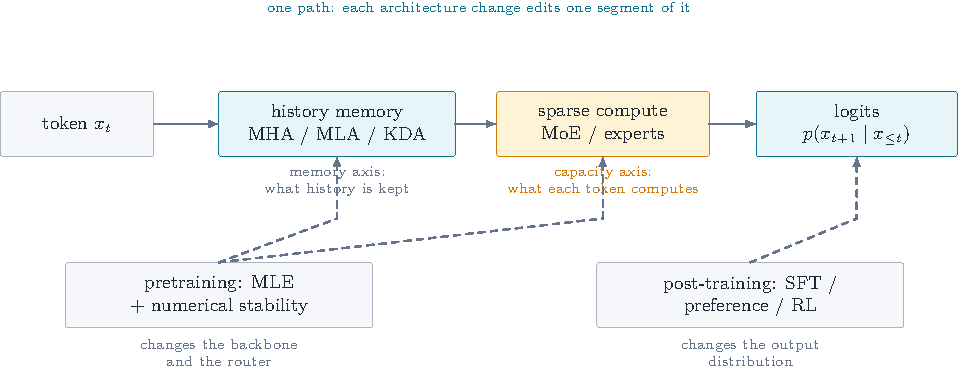
\includegraphics[width=\textwidth]{modern_llm_map.pdf}
\caption{沿一次 token 预测的信息流定位改动：历史读取决定能看见什么，专家路由决定执行哪些参数，后训练改变输出分布。}
\label{fig:modern-llm-map}
\end{figure}

\section{DeepSeek-V2：缓存短摘要，读取时生成 K/V}

这一节动的是第 1 条轴（历史读取），末尾顺带改动第 2 条轴（专家计算）。普通多头注意力在推理时为每个历史 token 缓存各个 head 的键和值（K/V）；上下文越长，要保存和读取的历史就越多。MLA 先把每个 token 的本层表示压成一份低维内容摘要，缓存这份摘要；位置键另走一条较窄的分支。后续 query 读取历史时，各 head 的内容键和值由对应位置的摘要计算得到~\cite{deepseekv2}。图 \ref{fig:mla-computation} 只画内容路径：从历史表示到短摘要，再从同一份摘要展开多个 head 的 K/V。历史位置的数量仍随序列增长，但每个位置保存的内容状态更小。

\begin{figure}[ht]
\centering
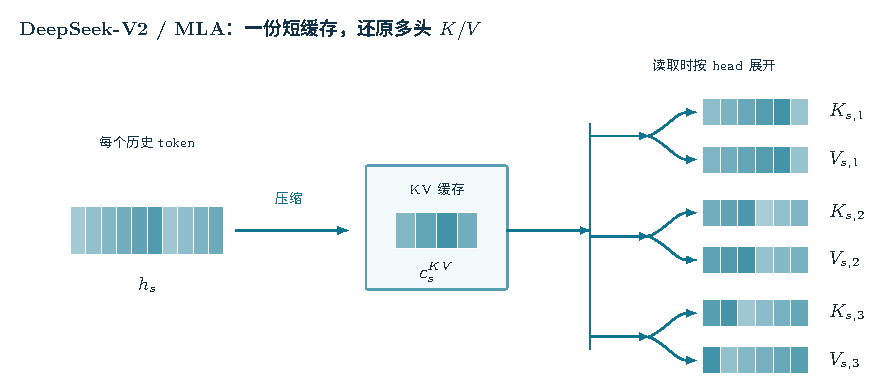
\includegraphics[width=\textwidth]{mla_computation.pdf}
\caption{图示 MLA 的内容路径：每个历史 token 的表示压缩为一份低维摘要，读取时由它重建各 head 的内容键和值。}
\label{fig:mla-computation}
\end{figure}

用 \(h_t\) 表示本层处理到的 token 的隐藏表示。第一步直接生成要缓存的短摘要；第二步从该摘要得到各 head 的内容键和值：
\begin{equation}
c_t^{KV}=W^{DKV}h_t,\qquad
k_{t,i}^{C}=W_{i}^{UK}c_t^{KV},\quad v_{t,i}^{C}=W_{i}^{UV}c_t^{KV}.
\label{eq:mla-cache}
\end{equation}
\(c_t^{KV}\) 由 \(h_t\) 直接计算，不需要先生成完整的逐 head K/V 再压缩。训练时，下一 token 损失穿过注意力和这些投影共同更新参数。推理时，新 token 到来后把 \(c_t^{KV}\) 和位置键写入缓存；后续 query 读取位置 \(t\) 时，再由缓存中的 \(c_t^{KV}\) 计算所需 head 的内容键和值，参与注意力计算~\cite{deepseekv2}。

V2 在 FFN 侧还把路由专家划得更细，并保留每个 token 都经过的共享专家~\cite{deepseekv2}。细专家提供更多可选组合，共享专家承接各 token 都需要的变换；Top-\(k\) 路由的基本机制已在第~\ref{sec:moe}~节给出。


\section{DeepSeek-V3：让专家自调负载，让表示多看一步}

这一节动的是第 2 条轴（专家计算）和第 4 条轴（训练信号）。稀疏路由会让热门专家收到过多 token，造成设备等待，也让冷门专家缺少训练。常见做法是把负载均衡写成辅助损失，随预测损失一起做梯度下降。DeepSeek-V3 则给每个专家一个独立的选择偏置~\cite{deepseekv3}：每个训练步骤结束，统计整个 batch 中各专家收到的 token 数；过载专家的偏置直接调低，欠载专家的偏置直接调高。这组偏置按负载统计规则更新，不通过梯度下降学习。下一轮路由时，偏置只改变 Top-\(k\) \textbf{选哪些专家}；选中专家的输出权重仍由原始亲和分数决定。图像化地看，各专家是并行服务队列，负载反馈调整下一轮的队列优先级，预测损失的梯度继续训练路由器和专家。

若 \(n_i\) 是本步分给专家 \(i\) 的 token 数，\(\bar n\) 是目标平均负载，反馈规则可简写为 \(b_i\leftarrow b_i+\gamma\operatorname{sign}(\bar n-n_i)\)。正负号分别对应给冷门专家加分、给热门专家减分；\(\gamma\) 控制每步改动的幅度。路由器产生的原始亲和分数仍通过预测损失学习，偏置 \(b_i\) 则执行这条独立的更新规则。

第二个改动落在监督位置。普通自回归训练让主模型读到 \(B\) 的表示预测下一个 token \(C\)；多 token 预测（Multi-Token Prediction，MTP）在主模型后接一个较轻的辅助 Transformer 模块，把这份表示和训练样本中真实的 \(C\) 合起来，经过一个 Transformer 块再预测 \(D\)~\cite{deepseekv3}。辅助模块与主模型共享词嵌入和输出头，新增的主要是一层 Transformer 和连接投影。

训练损失因此包括下一 token 预测（Next-Token Prediction，NTP）和 MTP 两部分，\(\mathcal L=\mathcal L_{\mathrm{NTP}}+\lambda\mathcal L_{\mathrm{MTP}}\)。NTP 损失沿主模型路径反传；更远一步的 MTP 损失经过辅助模块，也传回产生输入表示的主模型，同时更新两者。\(\lambda\) 调节额外监督的强度。图 \ref{fig:deepseek-v3-mtp} 把两条路径分开画出：辅助模块向前多探一步，主模型因而也收到来自更远 token 的训练信号。

\begin{figure}[H]
\centering
\begin{tikzpicture}[x=1cm,y=1cm]
  \node[tealblock,minimum width=28mm,minimum height=12mm] (main) at (2.0,1.0) {主模型\\读到 \(B\)};
  \node[softblock,minimum width=28mm,minimum height=10mm] (next) at (6.2,2.0) {预测下一个 \(C\)};
  \node[orangeblock,minimum width=39mm,minimum height=12mm] (aux) at (6.2,0) {真实 \(C\) + 辅助 Transformer\\预测更远的 \(D\)};
  \node[tealblock,minimum width=31mm,minimum height=10mm] (ntploss) at (11.6,2.0) {NTP 损失\\更新主模型};
  \node[orangeblock,minimum width=43mm,minimum height=12mm] (mtploss) at (11.6,0) {MTP 损失\\更新辅助模块与主模型};
  \draw[flow] (main.north east) -- (next.west);
  \draw[flow] (main.south east) -- (aux.west);
  \draw[flow] (next.east) -- (ntploss.west);
  \draw[flow] (aux.east) -- (mtploss.west);
\end{tikzpicture}
\caption{V3 的两路训练信号：主模型预测下一 token，较轻的辅助 Transformer 模块预测再下一 token；MTP 损失也回传到主模型。}
\label{fig:deepseek-v3-mtp}
\end{figure}

推理时，MTP 模块还可以快速提出后续候选 token，再由主模型并行验证。这沿用推测解码的思路，有望减少逐 token 调用主模型的次数，进而加速生成~\cite{deepseekv3,leviathan2023speculative}。


\section{DeepSeek-V3.2：先选相关 token，再精算注意力}

这一节动的是第 1 条轴（历史读取）。MLA 用每个历史 token 的短摘要代替逐 head 的内容 K/V 缓存；若当前 query 仍须与全部历史做完整注意力，长上下文的匹配计算依然很大。DeepSeek 稀疏注意力（DeepSeek Sparse Attention，DSA）增加一个轻量的 Lightning Indexer~\cite{deepseekv32}。它读入当前 token 的隐藏表示 \(h_t\)，以及由各历史 token 的表示 \(h_s\) 预先生成的轻量索引键；先给整个历史的每个位置打分，再输出分数最高的 Top-\(k\) 位置。主注意力随后只读取这些位置对应的 MLA 缓存条目，完成精细匹配与聚合。

索引器把 \(h_t\) 投影为少量低维 query \(q^I_{t,j}\) 及其标量权重 \(\omega_{t,j}\)，把 \(h_s\) 投影为低维 key \(k^I_s\)。匹配分数经过整流线性单元（Rectified Linear Unit，ReLU）后，一次检索可概括为
\begin{equation}
I_{t,s}=\sum_j \omega_{t,j}\operatorname{ReLU}\!\left((q^I_{t,j})^\mathsf T k^I_s\right),\qquad
\mathcal S_t=\operatorname{TopK}_{s<t} I_{t,s}.
\label{eq:deepseek-dsa-index}
\end{equation}
分数 \(I_{t,s}\) 衡量当前 token 与历史位置 \(s\) 的粗略相关性。所有历史索引键可一起参与打分，得到分数向量 \(I_t=[I_{t,1},\ldots,I_{t,t-1}]\)。\(\mathcal S_t\) 是索引器交给主注意力的历史位置集合。低维打分扫描全历史，昂贵的主注意力只在这个集合上运行。

\begin{figure}[H]
\centering
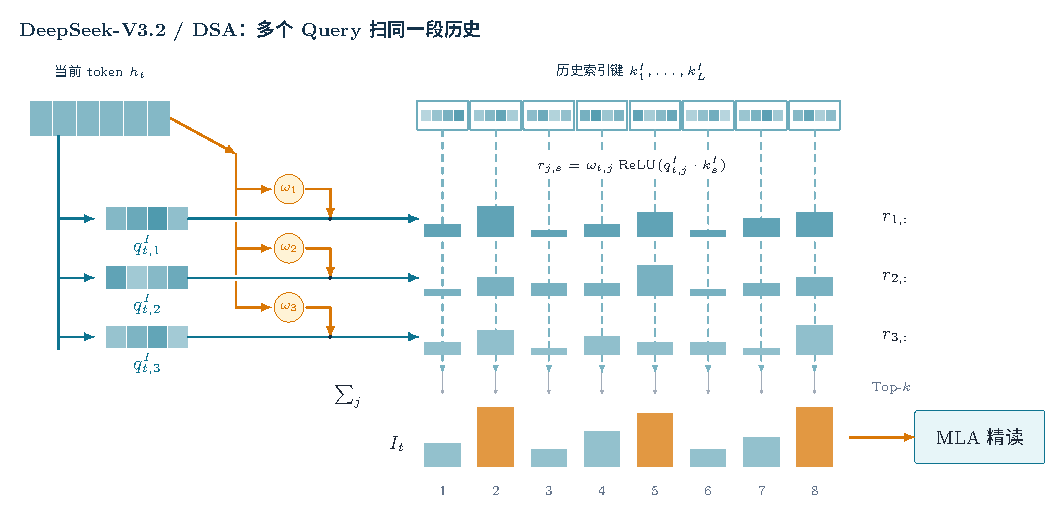
\includegraphics[width=\textwidth]{dsa_indexer.pdf}
\caption{上方每张小卡片是一个历史 token 的索引键。当前 token 生成多个 query 和对应的标量权重；每个 head 扫过同一段历史，形成一条非负的加权贡献。按历史位置逐列求和得到一条分数向量，橙色峰值是 Top-\(k\)，随后由 MLA 精读。}
\label{fig:deepseek-dsa}
\end{figure}

图 \ref{fig:deepseek-dsa} 中，当前 query 可以选到相距很远的历史位置。V2 的 MLA 缩小每张历史卡片，V3.2 的 DSA 则让主注意力只精读少数卡片：一次轻量扫描加少量精细计算，降低长上下文的注意力开销。

索引器的训练分两段。先保留稠密注意力并冻结主模型，把主注意力在历史各位置上的权重汇总成目标分布 \(p_{t,:}\)，让索引器的打分分布通过 \(\mathrm{KL}\bigl(p_{t,:}\Vert\operatorname{softmax}(I_{t,:})\bigr)\) 向它靠近；这一步教索引器识别主模型实际会关注的位置。随后启用 Top-\(k\) 稀疏选择，主模型继续用语言模型损失学习，索引器继续在选中位置上对齐主注意力的分布。两路训练信号分开：主模型沿预测损失更新，索引器沿分布对齐损失更新~\cite{deepseekv32}。


\Needspace{13\baselineskip}
\section{DeepSeek-R1：用可验证奖励选择推理轨迹}

这一节动的是第 4 条轴（训练信号）。语言模型的下一 token 损失学习怎样续写训练文本；数学答案和代码测试还提供了对整条回答的可验证反馈。DeepSeek-R1 在可验证任务的后训练中，把这类奖励与 GRPO 结合~\cite{deepseekr1}：同一道题由当前模型采样多条推理轨迹，判题器检查最终答案或代码结果，再比较同组轨迹的得分。若第 \(i\) 条轨迹得到奖励 \(r_i\)，核心比较量是式 \eqref{eq:grpo-advantage} 的组内标准化优势 \(A_i\)，它表示这条轨迹比同题其他尝试好多少。GRPO 按式 \eqref{eq:grpo-loss} 用它提高组内较好轨迹的生成概率，降低较差轨迹的生成概率，并约束策略不要一次改变过大。图像化地看，训练在同题的多条候选路径中反复强化成功路径；推理时，模型依据更新后的参数逐 token 生成推理过程和答案，判题器与组内比较只出现在训练环节。


\section{Kimi Linear：固定工作记忆加可翻查的历史}

这一节动的是第 1 条轴（历史读取）。完整注意力像一本可逐页翻查的档案：每个历史 token 都留下记录，长上下文的缓存和读取量随之增长。固定大小的递推状态像工作记忆，更新成本稳定，却会把许多过去的关联挤进同一份状态。Kimi Linear 沿层的深度方向重复“KDA、KDA、KDA、MLA”这一组：同一 token 依次经过三层 KDA，再经过一层 MLA。KDA 层维护固定大小的状态，MLA 层则保留可按内容寻找较早 token 的压缩历史~\cite{kimilinear}。

KDA 的关键是怎样维护这份有限状态。新 token 到来时，先按通道衰减过时关联，再用当前 key 从旧状态读出一个预测值，只把预测误差写回，最后由 query 读取更新后的状态。图 \ref{fig:kda-computation} 中的\textbf{衰减—纠错—读取}就是一次更新的全部动作：衰减控制保留多久，纠错减少新旧关联相互干扰。状态大小保持固定，周期性的 MLA 负责找回需要精确定位的历史细节。

\begin{figure}[H]
\centering
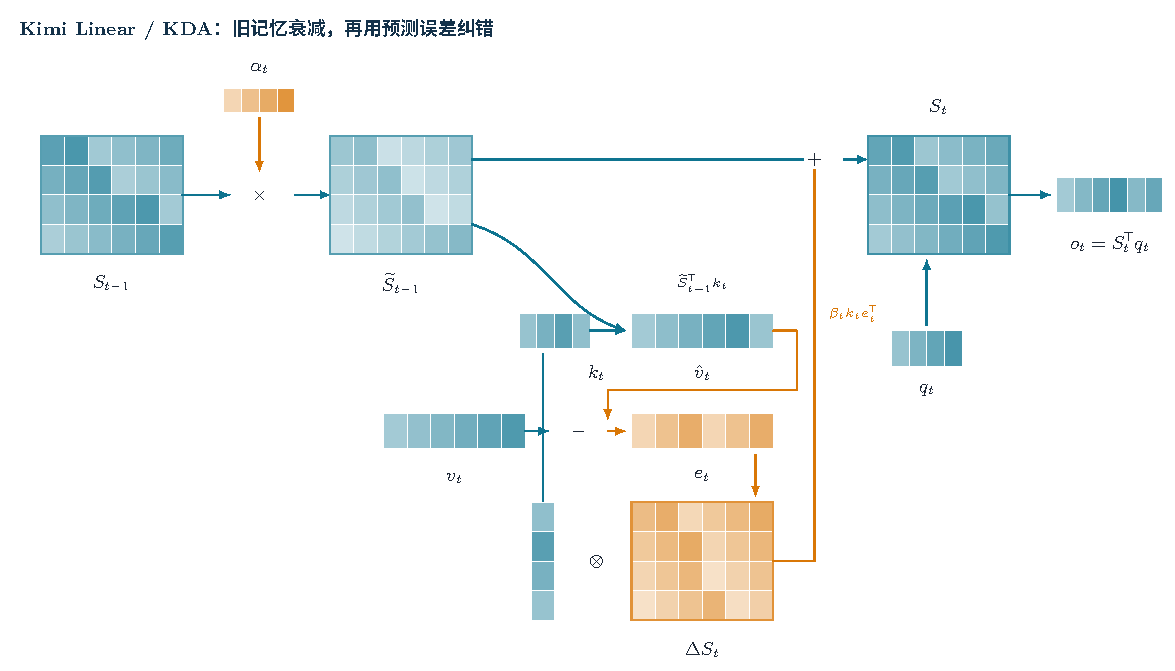
\includegraphics[width=\textwidth]{kda_computation.pdf}
\caption{KDA 把固定状态当作可修订的工作记忆：逐通道衰减旧关联，写入当前预测误差，再用 query 读取。}
\label{fig:kda-computation}
\end{figure}

图中的更新可以写成一条递推式。令 \(S_{t-1}\in\R^{d_v\times d_k}\) 为上一 token 留下的矩阵状态，方向与第 \ref{chap:transformer} 章线性注意力的 \(S_t\) 相同；\(\alpha_t\) 是每个 key 通道各自的保留比例，\(\beta_t\) 控制本次写入强度，\(q_t,k_t,v_t\) 来自当前输入：
\begin{equation}
\begin{aligned}
\widetilde S_{t-1}&=S_{t-1}\operatorname{Diag}(\alpha_t),\\
S_t&=\widetilde S_{t-1}+\beta_t\bigl(v_t-\widetilde S_{t-1}k_t\bigr)k_t^{\mathsf T},\qquad o_t=S_tq_t.
\end{aligned}
\label{eq:kda-update}
\end{equation}
第一行逐通道保留旧记忆；第二行先用当前 key 从旧状态读出预测 \(\widetilde S_{t-1}k_t\)，再把它与当前 token 的 value \(v_t\) 的差写回，最后用 query 读出 \(o_t\)。这正是图 \ref{fig:kda-computation} 的\textbf{衰减—纠错—读取}，也说明 KDA 如何用固定大小的状态持续修订键值关联~\cite{kimilinear}。

训练时，\(q_t,k_t,v_t,\alpha_t,\beta_t\) 都由可学习的投影和门控从输入产生；下一 token 损失通过 KDA 的状态更新及 MLA 层一起反传。长序列可分块并行计算块内结果，块与块之间传递状态。推理时每生成一个 token，KDA 层更新一次 \(S_t\)，MLA 层则把该 token 的短内容摘要和位置键加入缓存。前者的状态大小固定，后者承担按位置找回远处细节的任务~\cite{kimilinear}。


\section{DeepSeek-V4：多条残差流与分层历史摘要}

这一节动的是第 3 条轴（层间信息）和第 1 条轴（历史读取），末尾再涉及第 4 条轴（训练信号）。长模型同时沿两个方向积累信息：深度方向经过许多层，序列方向经过许多 token。DeepSeek-V4 分别改写这两条路径：流形约束超连接（Manifold-Constrained Hyper-Connections，mHC）让层间信息在多条残差流之间稳定混合；压缩稀疏注意力（Compressed Sparse Attention，CSA）与高度压缩注意力（Heavily Compressed Attention，HCA）让长历史以不同粒度被压缩和读取~\cite{deepseekv4}。下面分别看层间混合与历史读取。

\subsection{mHC：让深层有多条稳定的信息通道}

普通残差连接让每层在同一条表示流上继续累加。mHC 把层间状态展开成多条并行流：每层先从这些流中读出输入，算出注意力或 FFN 的新信息，再把新结果写回多条流~\cite{deepseekv4,mhc}。图 \ref{fig:mhc} 的上路负责本层读写，下路负责旧信息在各流间继续传递。

反复混合多条流容易放大或压低某些方向。mHC 约束流间混合权重为非负，且每行、每列的权重和接近 1；这样旧信息在各流间重新分配时保持受控的尺度。改动的亮点是增加层间信息通道，同时约束连续混合的稳定性；注意力和 FFN 仍处理通常宽度的输入。

把第 \(l\) 层的多条残差流记为 \(X_l\)，本层计算记为 \(\mathcal F_l\)，一次更新可写成
\begin{equation}
X_{l+1}=B_lX_l+C_l\mathcal F_l(A_lX_l),\qquad
B_l\mathbf 1=\mathbf 1,\quad \mathbf 1^{\mathsf T}B_l=\mathbf 1^{\mathsf T},\quad B_l\geq 0.
\label{eq:mhc-streams}
\end{equation}
\(A_l\) 从多条流读出本层输入，\(C_l\) 把新结果写回多条流，\(B_l\) 负责旧信息在流之间传递。训练时先从输入生成这些混合权重，再通过行、列归一化把 \(B_l\) 约束到式中的范围；预测损失通过整个读写过程反传。推理时，同一更新逐层作用于每个 token 的表示，无须改变注意力和 FFN 的内部宽度~\cite{deepseekv4,mhc}。

\begin{figure}[ht]
\centering
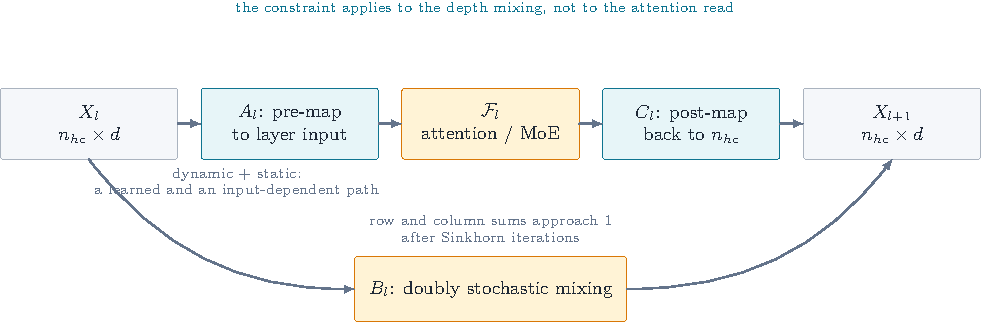
\includegraphics[width=\textwidth]{mhc.pdf}
\caption{从单条残差流到多条并行流：mHC 从多流读入子层，把新输出写回多流，并约束旧流之间的混合。}
\label{fig:mhc}
\end{figure}

\subsection{CSA/HCA：给长历史建目录和摘要}

把全部历史 token 逐一交给全局注意力，长上下文的匹配和缓存代价会不断增加。CSA 把短窗口压成较细的历史条目，再用 Lightning Indexer 找出与当前 query 最相关的少数条目；HCA 把更长的窗口压成更少的粗条目，可直接读取这些全局摘要~\cite{deepseekv4}。滑动窗口注意力（Sliding Window Attention，SWA）保留最近 token 的原始细节。这里的索引器选择压缩后的条目；V3.2 的 DSA 则选择每个历史 token 对应的 MLA 条目。

两条压缩路径共享一个基本动作：在窗口 \(W_i\) 内为各位置产生可学习的逐通道权重，再汇成一个缓存条目 \(\bar c_i=\sum_{s\in W_i}a_{i,s}\odot c_s\)，其中每个通道上的权重和为 1。CSA 的细条目吸收相邻窗口的信息，并在条目之间做 Top-\(k\) 选择；HCA 把更大的窗口压成粗条目，直接对全部粗条目做注意力。压缩权重随语言模型目标一起训练，CSA 的索引器先参考稠密注意力学习相关位置，再随稀疏注意力训练。推理时，新 token 逐步写入压缩历史；query 同时读取选中的细条目、全局粗条目和近期原始 token~\cite{deepseekv4}。

图 \ref{fig:csa-hca} 可以按\textbf{目录、摘要、近期原文}来读：CSA 先按目录挑选相关旧片段，HCA 给出较粗的全局概览，SWA 的局部窗口负责眼前细节。三种粒度一起降低长历史的直接搜索量，同时保留远处相关内容和近处精确信息。

\begin{figure}[ht]
\centering
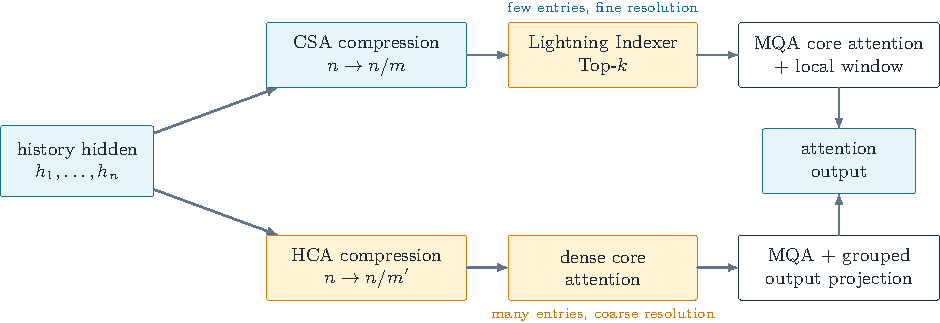
\includegraphics[width=\textwidth]{csa_hca.pdf}
\caption{CSA 在较细的压缩条目上做内容选择；HCA 读取更粗的全局摘要；局部窗口保留最近细节。}
\label{fig:csa-hca}
\end{figure}

\subsection{多领域后训练与在线蒸馏}

DeepSeek-V4 先在不同任务上分别后训练领域专长模型，再用第 \ref{sec:distillation} 节的多教师 on-policy 蒸馏把它们合进一个统一模型~\cite{deepseekv4}：统一模型在各领域的提示上自己生成回答，由该领域的专长模型在这些回答的前缀上给出下一 token 分布，按式 \eqref{eq:multi-teacher-opd} 更新，参数更新后重新采样。推理时只部署统一模型。

\section{Kimi K3：沿序列、深度和专家三处继续改进}

这一节沿第 1、3、2 条轴依次改动。Kimi K3 延续 Kimi Linear 的固定状态与可寻址历史组合，再处理三个新的限制：长序列递推的数值稳定、深层对早期表示的访问，以及大量专家之间的通信~\cite{kimik3}。图 \ref{fig:kimi-k3-block} 的上排是序列路径，下排是深度路径；专家模块放在每层 FFN 的位置。下文的注意力残差（Attention Residuals，AttnRes）处理跨层读取，稳定潜空间专家混合（Stable Latent Mixture of Experts，Stable LatentMoE）处理专家计算。

\begin{figure}[H]
\centering
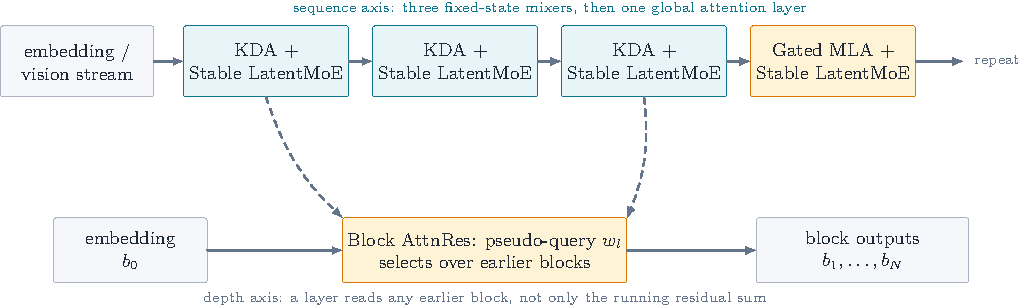
\includegraphics[width=\textwidth]{kimi_k3_block.pdf}
\caption{K3 在三处动手：KDA/Gated MLA 管序列历史，AttnRes 管跨层读取，Stable LatentMoE 管专家计算。}
\label{fig:kimi-k3-block}
\end{figure}

\subsection{序列：稳定的 KDA 与可控的全局读取}

KDA 的递推要在很长的序列上重复衰减与写入。K3 给衰减设定下界，避免反复更新时数值尺度走向极端；这提高长序列训练的稳定性。周期性的全局层继续使用 MLA，让模型直接找回较早的相关位置~\cite{kimik3}。全局注意力读出历史后，Gated MLA 再根据当前 token 对各输出通道加门控：相关通道多写入当前表示，干扰较大的通道少写入。图 \ref{fig:kimi-k3-block} 上排的三个 KDA 层与一个 Gated MLA 层体现了固定状态和全局读取的分工。

令 \(z_{t,j}\) 为 KDA 第 \(j\) 个 key 通道经过可学习缩放的衰减分数，K3 用 \(g_{t,j}=g_{\min}\operatorname{sigmoid}(z_{t,j})\)、\(\alpha_{t,j}=e^{g_{t,j}}\) 生成式 \eqref{eq:kda-update} 中的保留比例，其中 \(g_{\min}<0\)。这样 \(\alpha_{t,j}\) 有正的下界，分块并行训练时连续衰减的数值范围受到控制。对 MLA 读出的 \(\widetilde o_t\)，门控输出可写为 \(y_t=W_o[\operatorname{sigmoid}(W_gx_t)\odot\widetilde o_t]\)：当前 token 决定哪些历史通道进入下一层。训练时这些门控随下一 token 损失学习；推理时 KDA 继续逐 token 更新固定状态，MLA 缓存仍保留可按位置读取的历史~\cite{kimik3}。

\subsection{深度：AttnRes 按需翻回早期层}

普通残差让信息逐层累加；AttnRes 则保留较早层块为同一 token 产生的输出，并用它们组成当前层的输入~\cite{kimik3,attnres}。当前层 \(l\) 有一个训练得到的查询向量 \(w_l\)：它分别与各块输出的归一化表示做内积，得到每个块的匹配分数，再对所有可访问块的分数做 softmax。分数越高，该块输出在当前层输入中占的权重越大。这意味着，同一当前层面对不同 token 时，叠加先前各层输出所用的权重也可能不同；本层计算产生的新输出又成为更深层可读取的候选。图 \ref{fig:k3-attnres-depth} 将这条从已有输出到当前输入、再到新输出的路径画出来。这些块权重可以用来查看当前层主要读取了哪些较早的层。

\begin{figure}[ht]
\centering
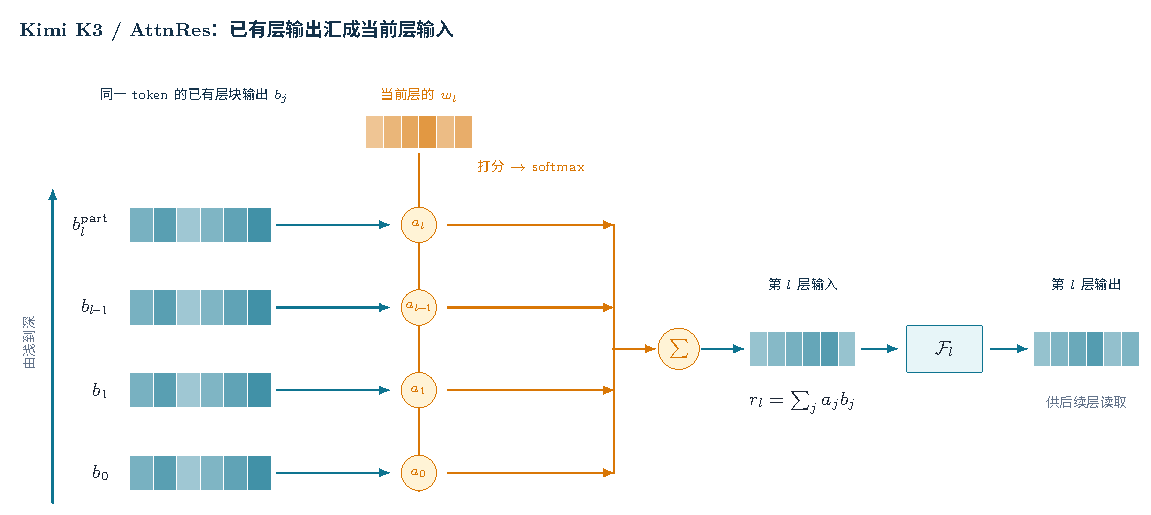
\includegraphics[width=\textwidth]{attnres_depth.pdf}
\caption{已有层块输出按当前层算出的权重汇合成输入 \(r_l\)，本层计算再产生新输出；图中的 \(a_j\) 是 \(a_{l,j}\) 的简写。}
\label{fig:k3-attnres-depth}
\end{figure}

\Needspace{9\baselineskip}
令 \(b_j\) 表示较早层块的输出或当前块已完成的部分，\(\mathcal B_l\) 是当前层可访问的块集合。打分、归一化和组成当前层输入依次写为
\begin{equation}
\begin{aligned}
s_{l,j}&=w_l^{\mathsf T}\operatorname{RMSNorm}(b_j),\\
a_{l,j}&=\frac{\exp(s_{l,j})}{\sum_{i\in\mathcal B_l}\exp(s_{l,i})},\\
r_l&=\sum_{j\in\mathcal B_l}a_{l,j}b_j.
\end{aligned}
\label{eq:attnres-block}
\end{equation}
\(\operatorname{RMSNorm}(b_j)\) 用来计算分数，控制不同层块输出的尺度差异；真正加权相加的是块输出 \(b_j\) 本身。\(r_l\) 是第 \(l\) 层的输入，经过本层计算后才产生新的输出。V4 的 mHC 同时维护多条并行残差流，K3 的 AttnRes 则从较早深度按需读取。

\subsection{专家：先压窄，再送入路由专家}

普通专家并行把模型宽度的表示发往选中的专家，跨设备传输随激活专家数增加。Stable LatentMoE 先把路由分支压到较窄的潜空间，让专家在这个空间计算，再把聚合结果映射回模型宽度；共享专家仍接收完整表示~\cite{kimik3}。若输入 \(x\in\mathbb R^d\)、压缩表示 \(z\in\mathbb R^\ell\) 且 \(\ell<d\)，\(E_i\) 是路由专家、\(p_i\) 是选中专家的混合权重，两条路径合起来可写为
\begin{equation}
z=W^{\downarrow}x,\qquad
u=\sum_{i\in\mathcal T(x)}p_iE_i(z),\qquad
y=\sum_j E_j^{\mathrm{shared}}(x)+W^{\uparrow}\operatorname{RMSNorm}(u).
\label{eq:k3-latent-moe}
\end{equation}
\begin{figure}[ht]
\centering
\begin{tikzpicture}[x=1cm,y=1cm]
  \node[softblock,minimum width=18mm,minimum height=9mm] (x) at (0.9,0) {输入 \(x\in\mathbb R^d\)};
  \node[tealblock,minimum width=25mm,minimum height=10mm] (down) at (3.4,1.25) {降维 \(W^{\downarrow}\)\\\(z\in\mathbb R^\ell\)};
  \node[orangeblock,minimum width=29mm,minimum height=10mm] (route) at (6.9,1.25) {Top-\(k\) 路由\\专家处理 \(z\)};
  \node[tealblock,minimum width=25mm,minimum height=10mm] (mix) at (10.25,1.25) {加权聚合\\RMSNorm};
  \node[tealblock,minimum width=22mm,minimum height=10mm] (up) at (13.1,1.25) {升维 \(W^{\uparrow}\)\\回到 \(d\) 维};
  \node[orangeblock,minimum width=33mm,minimum height=10mm] (shared) at (6.9,-1.15) {共享专家处理完整 \(x\)};
  \node[softblock,minimum width=17mm,minimum height=9mm] (out) at (13.1,-1.15) {相加得 \(y\)};
  \draw[flow] (x.north east) -- (down.west);
  \draw[flow] (down.east) -- (route.west);
  \draw[flow] (route.east) -- (mix.west);
  \draw[flow] (mix.east) -- (up.west);
  \draw[flow] (x.south east) -- (shared.west);
  \draw[flow] (shared.east) -- (out.west);
  \draw[flow] (up.south) -- (out.north);
\end{tikzpicture}
\caption{Stable LatentMoE 的两条路径：路由专家接收低维表示 \(z\)，共享专家接收完整表示 \(x\)，两路输出回到同一宽度后相加。}
\label{fig:k3-latent-moe}
\end{figure}

图 \ref{fig:k3-latent-moe} 中，路由专家收到较窄的任务摘要 \(z\)，跨设备传送的也是这份低维表示。聚合后的归一化控制路由分支的尺度；专家内部的 SiTU-GLU 用平滑的 \(\beta\tanh(a/\beta)\) 限制大激活。训练时，下一 token 损失更新降维与升维投影、路由器、共享专家和选中的路由专家；Quantile Balancing 则根据一批 token 的路由分数分位数直接调整下一步的专家选择偏置，使各专家接近目标负载。推理时依据路由分数与训练结束时保留的偏置选专家，只向路由专家传送低维 \(z\)，再把两条路径的结果相加~\cite{kimik3}。
